\lab{Image Compression (SVD)}{SVD}

\objective{Learn how to compute the compact SVD and explore the SVD as a method of image compression.}
\label{lab:SVD}



The theoretical use of the \emph{Singular Value Decomposition} or \emph{SVD} has long been appreciated.
In fact, the idea of a canonical way of decomposing a matrix was so alluring that the SVD was independently discovered by at least four people through use of both  integral equations and systems of linear equations.

However, it wasn't until Erhard Schmidt showed how the SVD could be a computational tool for providing low-rank approximations that the practical applications became apparent.
Since Schmidt's work, further devolpments have confirmed the importance of the SVD in both computational and theoretical applications.

\begin{comment}

The \emph{Singular Value Decomposition} is so important that it was discovered multiple times by different people in different ways.
The foundation work in systems of linear equations was laid by Gauss and Cauchy in the 1820's and later by Jacobi in 1846 with his work with the LU decomposition; however, the real work with the SVD started with Eugenio Beltrami.
In a paper he published in 1873 he was the first to work with the SVD; he was limited to real, square, nonsingular matrices with distinct singular values.
A year later, Camille Jordan published his own independent work that was more rigourus and avoided some of the pitfalls of Beltrami's research.
Together, Beltrami and Jordan are considered the codiscoverers of the singular value decomposition.

Later, James Joseph Sylvester independently presented an iterative algorithm and a rule for carrying out the reduction in 1889.
This rule was essentially Beltrami's work.
However Sylvester sent the note detailing his rule to the same  journal Jordan had published in, showing not just his ignorance of Jordan's and Beltrami's works but his perception of the SVD's importance.


The SVD's concurrent and independant derivation shows its importance as a theoretical tool, but it wasn't until Erhard Schmidt discovered a computational use for the SVD that the practical applications became apparent.
Schmidt used integral equations rather than linear equations to derive the SVD, but
his most important contribution was showing how the SVD could be a computational tool to obtain optimal, low-rank approximations.

Since Schmidt's work, further devolpments have confirmed the importance of the SVD in both practical and theoretical applications.
\end{comment}

\subsection*{Computing the SVD}


The Singular Value Decomposition separates a $m \times n$ matrix $A$ into two unitary matrices and a diagonal matrix.
This takes the form of 
\begin{equation*}
A = U \Sigma V^H
\end{equation*}
where $U$ and $V$ are square and unitary of sizes $m$ and $n$ respectively, and $\Sigma$ is diagonal and of size $m \times n$.
The values of $\Sigma$ are the \emph{singular values} of $A$, and are the square root of the eigenvalues of $A^HA$.
% if $A$ is square, are equal to the absolute value of the eigenvalues of $A$.
Commonly the singular values are listed in decreasing order. Thus we get

\begin{equation*}
\Sigma = \mbox{diag}(\sigma_1,\sigma_2,\ldots,\sigma_n)
\end{equation*}
where $\sigma_1 \geq \sigma_2 \geq \ldots \geq \sigma_n \geq 0$ are the singular values of $A$.

The \emph{compact SVD} is where the $r$ column vectors of $U$ and the $r$ row vectors of $V$ are calculated, cooresponding to the $r$ nonzero singular values.
We lose the decomposition of the nullspace of $A$, but can still regain the full matrix $A$.
It takes the form $A= U_1 \Sigma_1 V_1^H$ where $U_1$ is $m\times r$, $\Sigma_1$ is $r\times r$ and diagonal, and $V_1^H$ is $r\times n$.

The \emph{truncated SVD} is similar to the compact SVD, but instead of taking all the nonzero singular values, we only take the $k$ largest.
While this saves space, it means that we cannot recover the whole matrix.
Instead we have an approximation that shares the largest $k$ singular values.
We end up with $\widehat A = U_k\Sigma_k V_k^H$ where $\widehat A$ is an approximation of $A$, $U_k$ is $m\times k$, $\Sigma$ is $k \times k$ and diagonal, and $V_k^H$ is $k \times n$.

The only difference in computing the compact SVD verses the truncated SVD is the number of singular values we keep.
If we keep all the nonzero singular values, it is the compact SVD.
If we only keep some of the nonzero singular values, then it is the truncated SVD.

To compute the compact or truncated SVD:

\begin{itemize}
\item The singular values of $A$ are the square root of the eigenvalues of $A^HA$ and are sorted in descending order. These are the diagonal of $\Sigma$. For the compact SVD, keep all nonzero singular values. For the truncated SVD, keep the first $k$.
\item The columns of $V$ are the eigenvectors of $A^HA$, where the $i$th column matches the $i$th singular value.
\item The columns of $U$ are $U_i = \frac{1}{\sigma_i} AV_i$.
\end{itemize}

\begin{comment}
To calculate the SVD:
\begin{itemize}

\item Find $A^HA$

\item Find the eigenvalues and eigenvectors of $A^HA$.

\item Sort the eigenvalues in decreasing order.

\item The $i^{th}$ column of $V$, $V_i$, is the eigenvector corresponding to the $i^{th}$ eigenvalue.

\item Find the singular values by taking the square root of the eigenvalues.

\item The $i^{th}$ column of $U$ is $U_i = \frac{1}{\sigma_i} AV_i$.

\end{itemize}
\end{comment}

\begin{comment}
\begin{algorithm}
\begin{algorithmic}[1]
\caption{SVD for Full Rank Square Matrices.}
\label{Alg:svd_full}
\Procedure{SVD}{$A$}
\State $n \gets \shape{A}$
\State $eigs \gets$ eigenvalues$(A^HA)$
\State sort$(eigs)$
\State $V \gets$ eigenvectors$(A^HA)$
\State $svals \gets \sqrt{eigs}$
\State $U \gets \allocate{n,n}$
\For{$i=0\ldots n-1$}
      \State $U_i \gets  \frac{1}{svals[i]} AV_i$
\EndFor
\State $S \gets$ diag$(svals)$
\State \pseudoli{return} $U, S, V^H$
\EndProcedure
\end{algorithmic}
\end{algorithm}
\end{comment}

\begin{problem}
Write a function to calculate either the truncated SVD or the compact SVD.
Since the process is the same, we only need to write one function.

\begin{enumerate}
\item Find the eigenvalues and eigenvectors of $A^H A$.
\item Find the singular values of $A$.
\item Sort the singular values and only keep the greatest $r$.
\item Calculate $V$.
\item Calculate $U$.
\end{enumerate}

Check your function by calculating the compact SVD and seeing if $U_1\Sigma_1 V_1^H = A$ using \li{np.allclose()}.

Hint: While calculating the truncated SVD, you will need to sort the eigenvalues while keeping track of their associated eigenvectors. To accomplish this, use \li{np.argsort}.

\label{prob:calc_svd}
\end{problem}

If $A$ is full rank and square, it has $n$ nonzero singular values and this process gives us the full SVD.
If $A$ is not full rank or not square, we can compute the first $r$ columns of $U$ and $V$, where $r$ is the number of nonzero singular values, in this way.
To find the rest of the SVD, we can use Gram-Schmidt orthonormalization.

More specifically, let $r$ be the number of nonzero singular values.
If $r<n$ then we only have $r$ eigenvectors to fill $V$, which is a $n\times n$ matrix.
We find the remaining columns of $V$ by using Gram-Schmidt orthonormalization to finish the basis for $n$-space.
Similarly, if $r<m$ then we only have $r$ columns of $U$ so we use Gram-Schmidt orthonormalization to finish the basis for $m$-space.
The compact SVD does not have this problem because $U_1$ and $V_1$ only have $r$ columns, the remaining columns are the decomposition of the null spcae of the matrix, and are not included.
In this lab we calculate the compact SVD for simplicity.


\subsection*{Visualizing the SVD}

Recall that a matrix is one way to express a linear transformation.
A $m\times n$ matrix sends points from $\mathbb{R}^n$ to $\mathbb{R}^m$.
These transformations are a mix of rotations and rescalings.
The SVD decomposes these transformations into their individual parts.
$V^H$ is a rotation, $\Sigma$ a rescaling along the principal axes, and $U$ is another rotation.


\begin{figure}
\centering
\begin{subfigure}[b]{.49\textwidth}
  \centering
  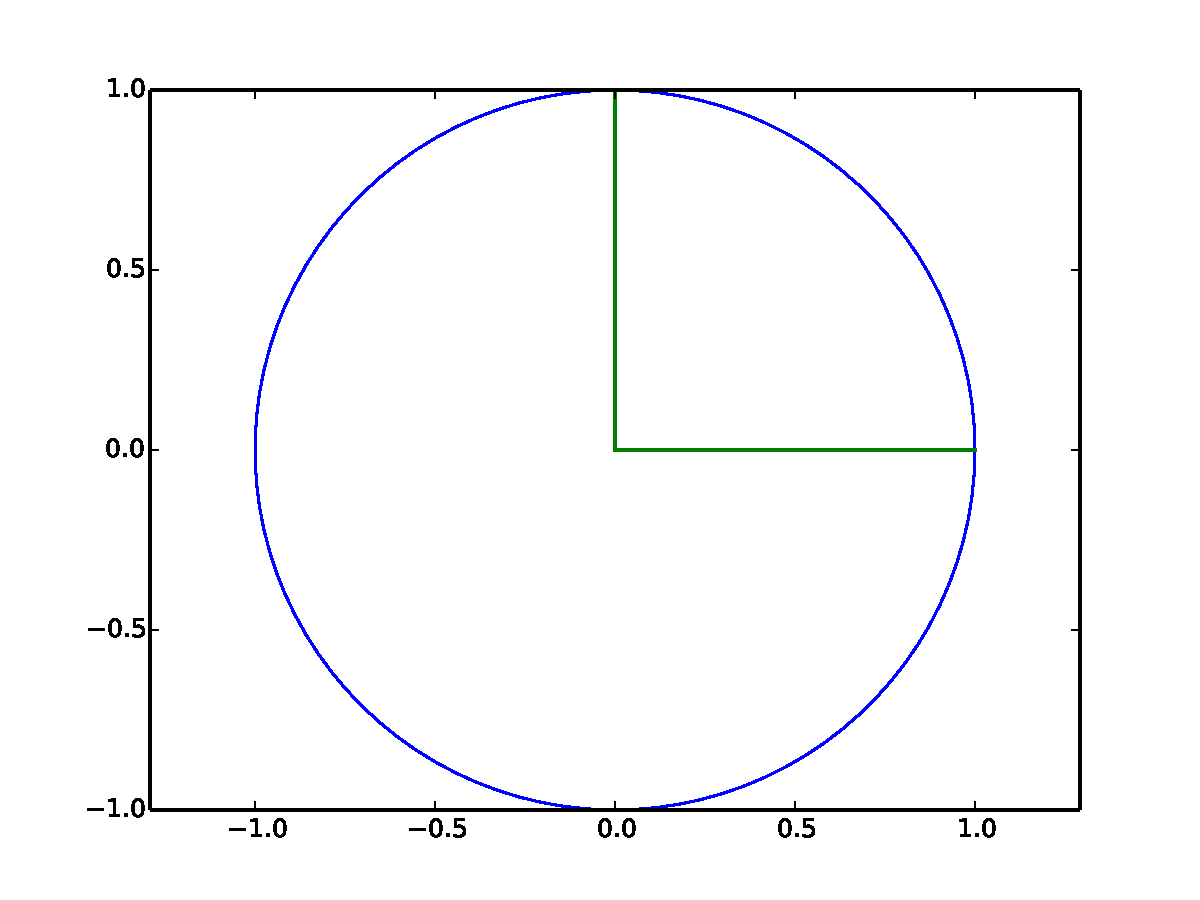
\includegraphics[width=\textwidth]{unit_circle.pdf}
  \caption{The unit circle, $S$, with two unit vectors.}
\end{subfigure}
\begin{subfigure}[b]{.49\textwidth}
  \centering
  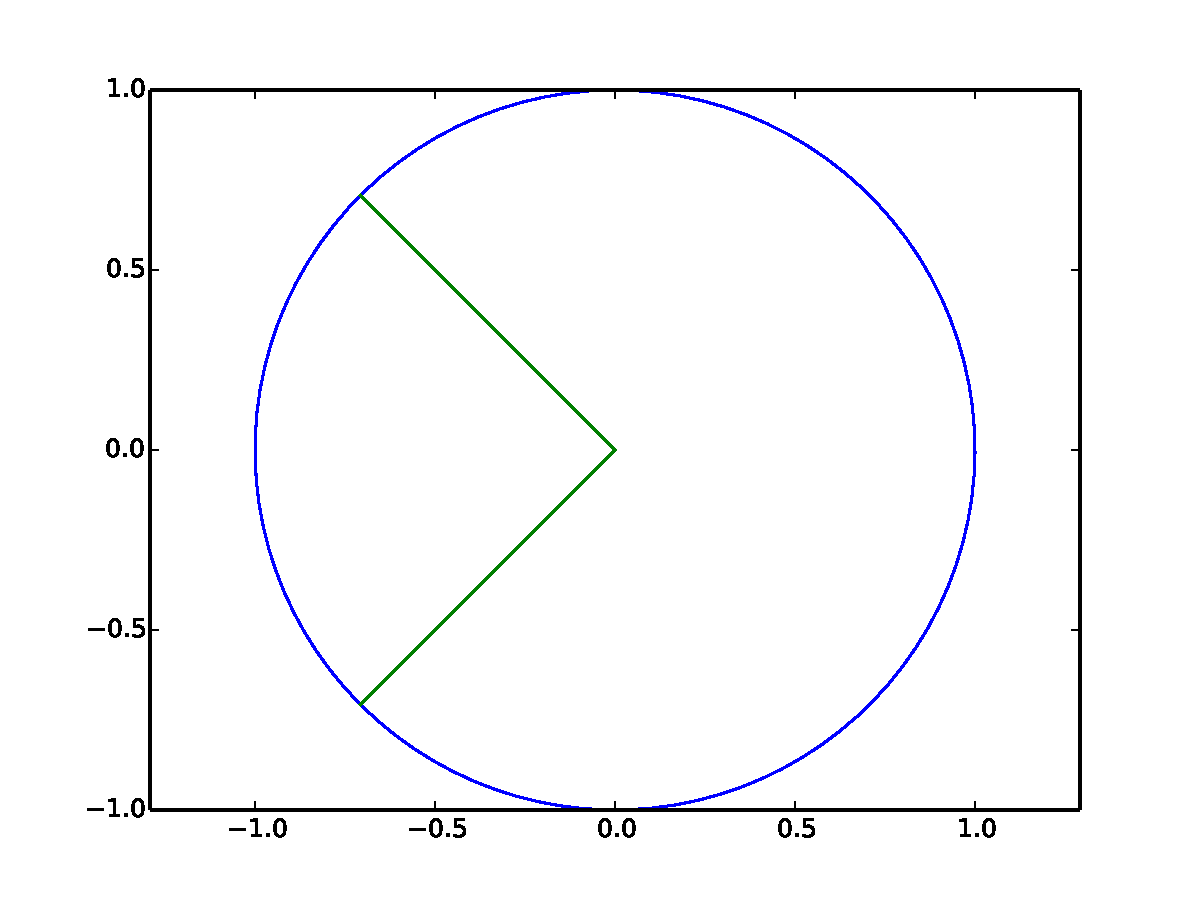
\includegraphics[width=\textwidth]{vcircle.pdf}
  \caption{$V^HS$}
  %\label{fig:svals_plot}
\end{subfigure}
\begin{subfigure}[b]{.49\textwidth}
  \centering
  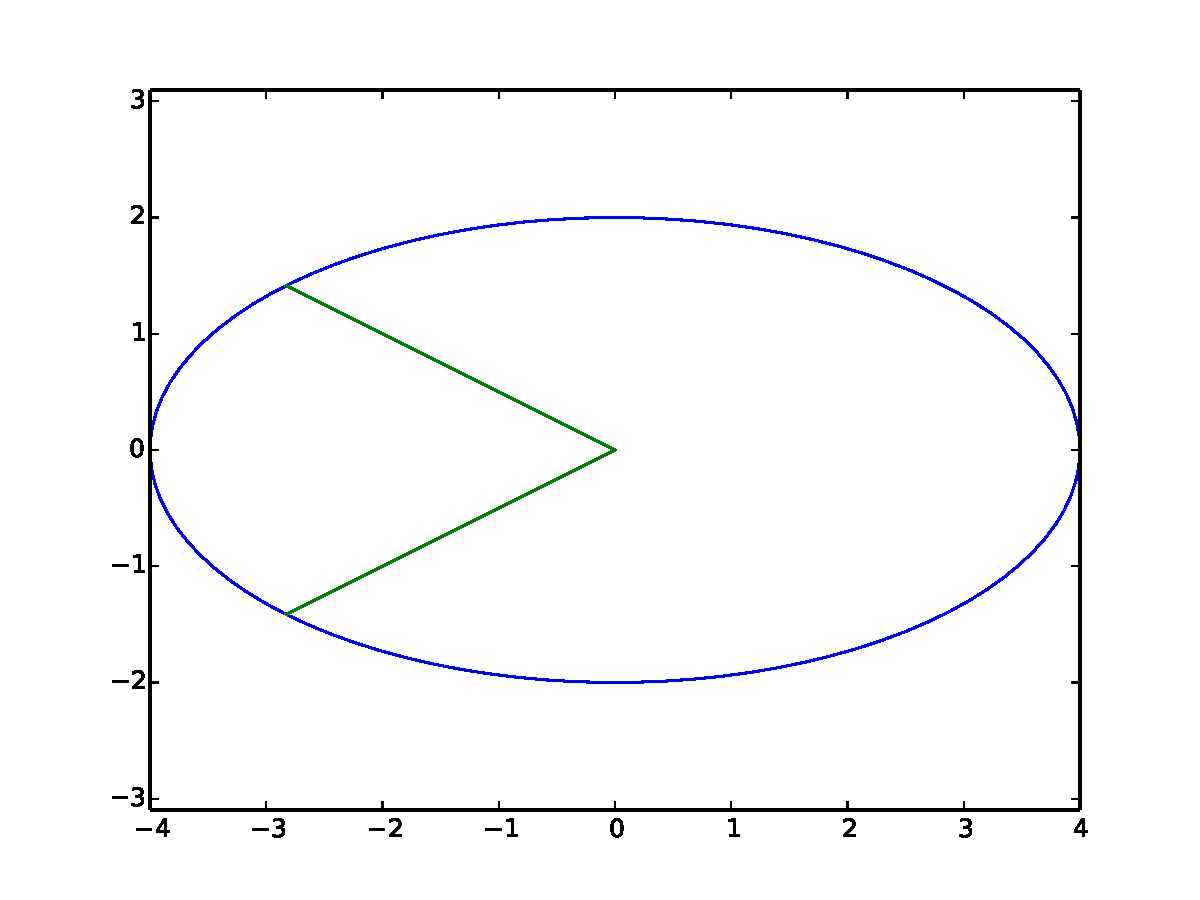
\includegraphics[width=\textwidth]{svcircle.pdf}
  \caption{$\Sigma V^H S$}
  %\label{fig:svals_plot}
\end{subfigure}
\begin{subfigure}[b]{.49\textwidth}
  \centering
  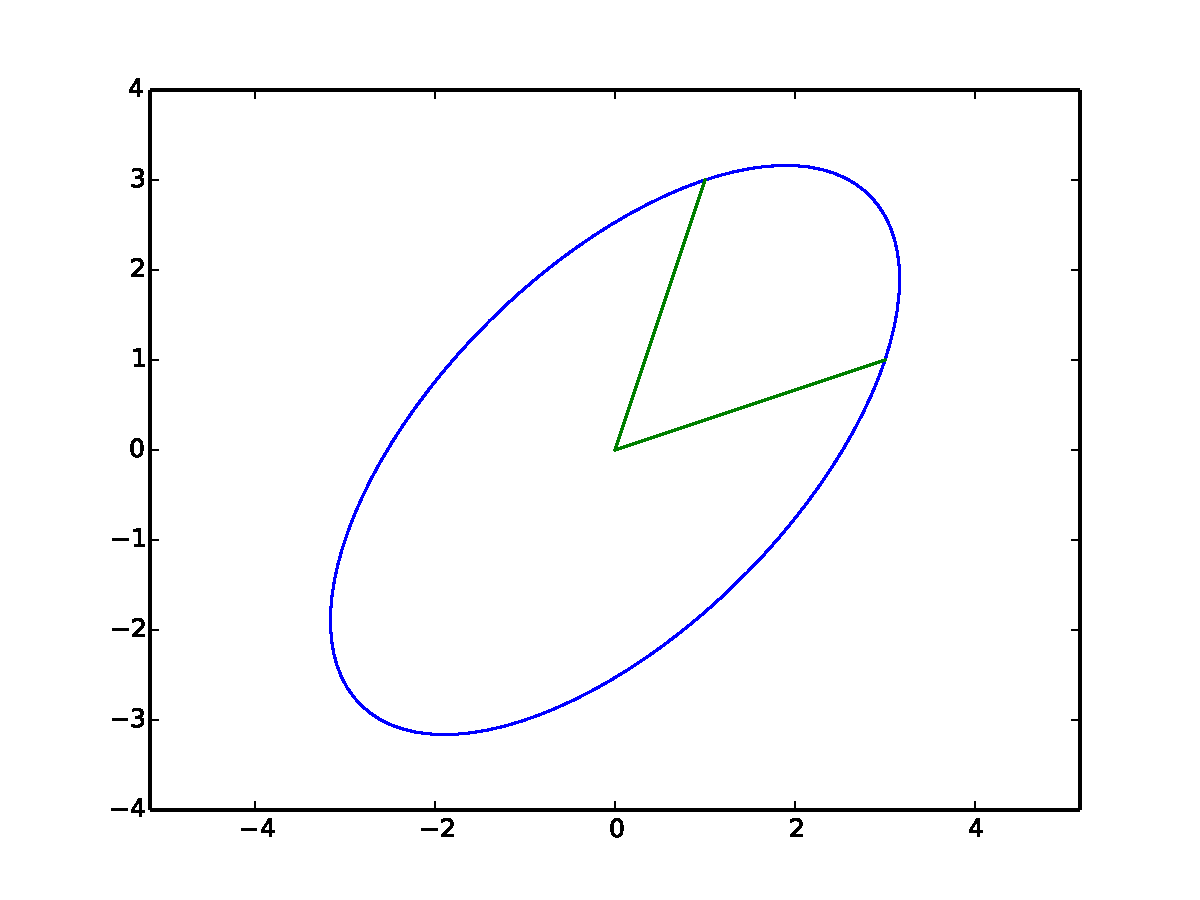
\includegraphics[width=\textwidth]{full_transformation.pdf}
  \caption{$U \Sigma V^H S$}
  %\label{fig:svals_plot}
\end{subfigure}
\caption{Each step in transforming the unit circle and two unit vectors using the matrix $A$.}
\label{fig:sol1}
\end{figure}

\begin{problem}
If $S$ are the points on the unit circle, $U\Sigma V^HS$ is equivalent to $AS$ where $U\Sigma V^H$ is the SVD of $A$. Using either your SVD from problem \ref{prob:calc_svd} or from scipy.linalg.svd, plot each part of the transformation of the matrix
\begin{equation}
A =  \begin{pmatrix}3 & 1\\1 & 3\end{pmatrix}.
\end{equation}

Your solution should show $S$, $V^HS$, $\Sigma V^HS$, and $U\Sigma V^HS$.
Since $A$ is square and full rank, the compact SVD is equal to the full SVD.
You solution should look like Figure \ref{fig:sol1}

The \li{circle.npz} dataset contains a set of points on the unit circle and a set of unit vectors. You can access the circle by loading the \li{"circle"} file. You can access the unit vectors by loading the \li{"unit_vectors"} file. These points are stored as a numpy array of points in $\mathbb{R}^2$ with the first row being all the x-coordinates and the second row being all the y-coordinates.
\end{problem}


\subsection*{Image Data Compression}

In this lab, we explore how the SVD can be used to compress image data.
Recall that an image is simply a matrix where each position is the color value for the pixel in that position.
The SVD lets us choose how much information to keep, and what information is most important.
Larger eigenvalues correspond to columns of $U$ and $V$ that contain more information, while smaller eigenvalues correspond to less important columns.
This idea is used in many areas of applied mathematics including signal processing, statistics, semantic indexing (search engines), and control theory.


\subsection*{Low rank data storage}
If the rank of a given matrix is significantly smaller than its dimensions, the compact SVD offers a way to store $A$ with less memory.
Without the SVD, an $m\times n$ matrix requires storing $mn$ values.
By decomposing the original matrix into the compact SVD, $U_1$, $\Sigma_1$ and $V_1$ together require $mr+r+nr$ values.
Thus if $r$ is much smaller than both $m$ and $n$, we can obtain considerable efficiency.
For example, suppose $m=100$, $n=200$ and $r=20$.
Then the original matrix would require storing $20,000$ values whereas the compact SVD only requires storing $6020$ values.

\subsection*{Low rank approximation}
The truncated SVD is useful in approxiamating a matrix with one of lower rank.
By only keeping the first $k$ singular values, we can create an approximation $\widehat A = U_k\Sigma_k V_k^H$.

\begin{comment}
We can also calculate $\widehat A$ by finding the full SVD, and setting all singular values after the $k$th to zero.
Thus the modified $\Sigma$ would be
\begin{equation*}
\Sigma_{\widehat A} = \mbox{diag}(\sigma_1,\sigma_2,\ldots,\sigma_s,0,\ldots,0).
\end{equation*}
Multiplying this matrix with the original $U$ and $V^H$ will give the same $\widehat A$ that was found by computing the truncated SVD directly.
\end{comment}



The \li{scipy.linalg} module has a convenient method to calculate the SVD of a given matrix. We can use
this method to create a lower-rank approximation of a given matrix. Execute the following code.
\begin{lstlisting}
>>> import numpy as np
>>> import scipy.linalg as la
>>> A = np.array([[1,1,3,4], [5,4,3,7], [9,10,10,12], [13,14,15,16], [17,18,19,20]])
>>> U,s,Vh = la.svd(A, full_matrices=False)
\end{lstlisting}
In that last line of code, we included the keyword argument \li{full_matrices=False} to calculate the
compact SVD rather than the full SVD. The arrays \li{U} and \li{Vh} correspond to the matrices
$U_1$ and $V_1^H$ discussed earlier in the lab. The array \li{s} simply gives the nonzero singular values
of the matrix \li{A}, and we can find the rank of \li{A} by inspecting the number of entries in \li{s} (in this
example, we have a rank 4 matrix). 

Next, we calculate a rank 3 approximation.
We take the first three singular values and the first three columns of \li{U} and first three rows of \li{Vh}.

We omit the last singular value from the calculation along with the last column of \li{U} and last row of \li{Vh}.

\begin{lstlisting}
>>> S = np.diag(s[:3])
>>> Ahat = U[:,:3].dot(S).dot(Vh[:3,:])
>>> la.norm(A-Ahat)
\end{lstlisting}
Note that $\widehat A$ is ``close'' to the original matrix $A$, but that its rank is 3 instead of 4. More
precisely, $\widehat A$ is the best rank 3 approximation of $A$ with respect to both the induced 2-norm and
the Frobenius norm. 

\begin{problem}
Write a function \li{svd_approx} that takes as input a matrix $A$ and a positive integer $k$ and returns 
the best rank $k$ approximation to $A$ with respect to the induced 2-norm.
\label{prob:svd_approx}
\end{problem}


\begin{comment}
The reduced form of the SVD also provides a way to approximate a matrix with another one of lower rank.
This idea is used in many areas of applied mathematics including signal processing, statistics, semantic indexing (search engines), and control theory.
If we are given a matrix $A$ of rank $r$, we can find an approximate matrix $\widehat A$ of rank $s<r$ by taking the SVD of $A$ and setting all of its singular values after $\sigma_s$ to zero, that is,
\begin{equation*}
\Sigma_{s} = \mbox{diag}(\sigma_1,\sigma_2,\ldots,\sigma_s,0,\ldots,0)
\end{equation*}
and then multiplying the matrix back together again.
The more singular values we keep, the closer our approximation is to $A$.
The number of singular values we decide to preserve depends on how close of an approximation we need and what our size requirements are for $U_1$, $\Sigma_{\widehat A}$, and $V_1$.
Try plotting the singular values.
\end{comment}

\subsection*{Application to Imaging}

Sometimes there is not enough available bandwidth to transmit a full resolution photograph.
You aim to reduce the amount of data that needs to be transmitted from a remote location such that loss of image detail is minimal, but the amount of data that needs to be sent has reduced as much as possible.
In Figure \ref{fig:hubble} we present an image and a plot of its singular values.
Matrix rank is on the x-axis and the singular values are on the y-axis.
Note that the SVD orders the singular values from greatest to least.
The more singular values we keep, the closer the approximation but the more data we have to store.
By looking at the graph in Figure \ref{fig:svals_plot} we can have a rough idea of how many singular values we need to preserve to have a good approximation of $A$.
The matrix rank of the image is $670$.
However, we could easily approximate the image using only the first half of the singular values as the plot shows that all the values after are miniscule.


%The greatest singular values contribute most to the image while the smallest singular values hardly contribute anything to the final approximation. %said this earlier

In Figure \ref{fig:rankvalues}, we can see different rank approximations of the image in Figure \ref{fig:hubble}.

\begin{figure}
\centering
\begin{subfigure}[b]{.49\textwidth}
\centering
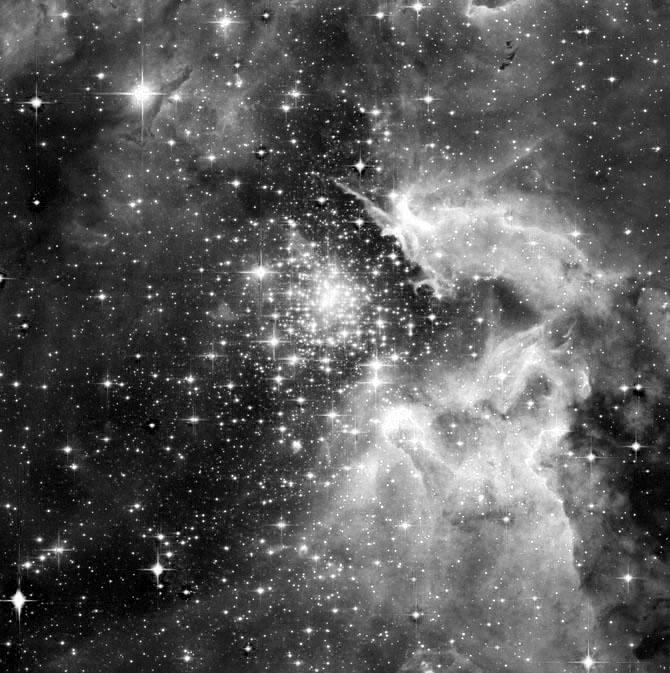
\includegraphics[width=\textwidth]{hubble_red}
\caption{NGC 3603 (Hubble Space Telescope).}
\end{subfigure}
\begin{subfigure}[b]{.49\textwidth}
\centering
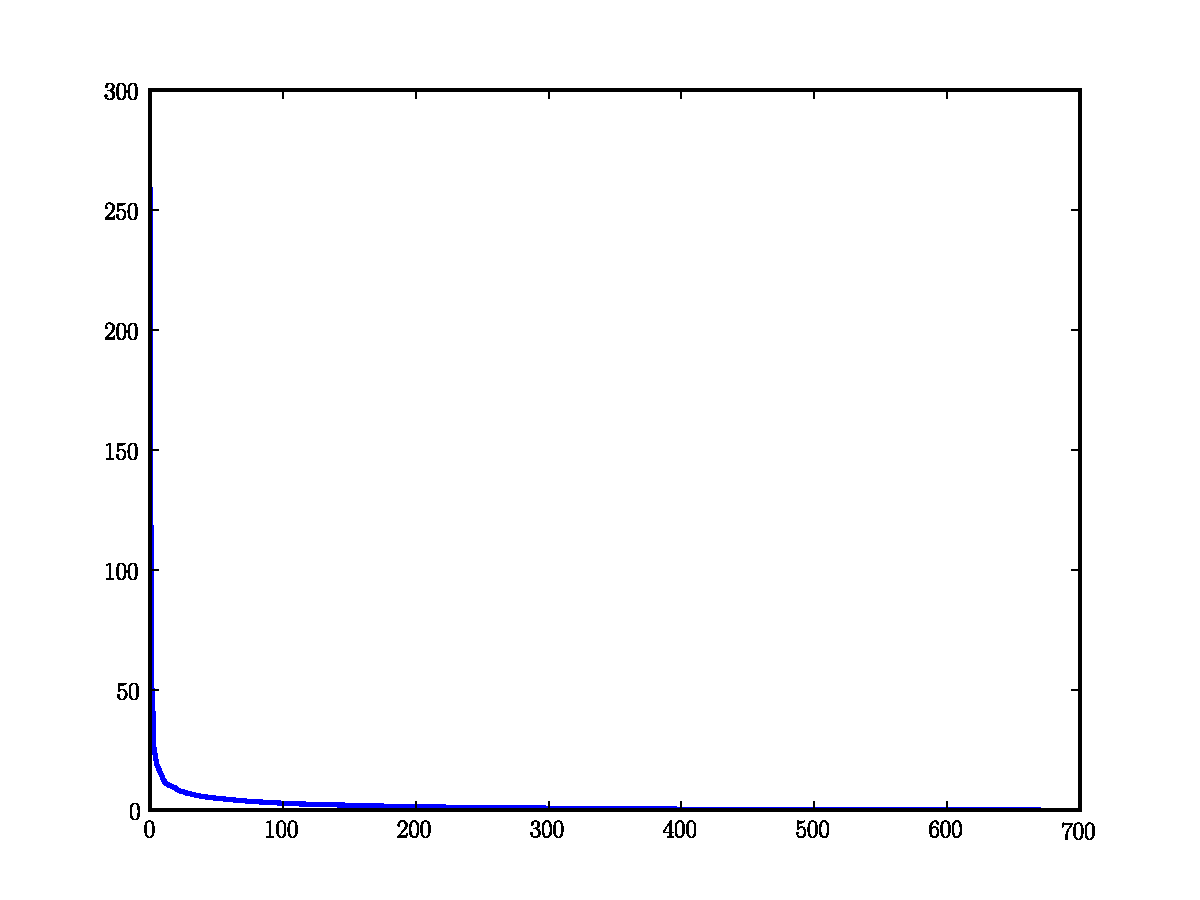
\includegraphics[width=\textwidth]{hubble_svals}
\caption{Singular values from greatest to smallest.}
\label{fig:svals_plot}
\end{subfigure}
\caption{An image and its singular values.}
\label{fig:hubble}
\end{figure}

\begin{figure}
\centering
\begin{subfigure}[b]{.25\textwidth}
\centering

\includegraphics[width=\textwidth]{rank1.jpg}
\caption{Rank 1}
\end{subfigure}
\begin{subfigure}[b]{.25\textwidth}
\centering
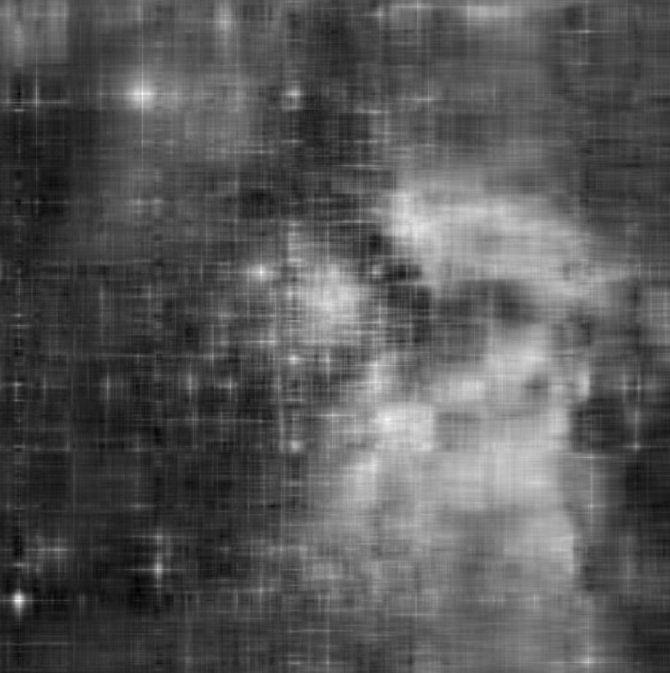
\includegraphics[width=\textwidth]{rank14.jpg}
\caption{Rank 14}
\end{subfigure}

\begin{subfigure}[b]{.25\textwidth}
\centering
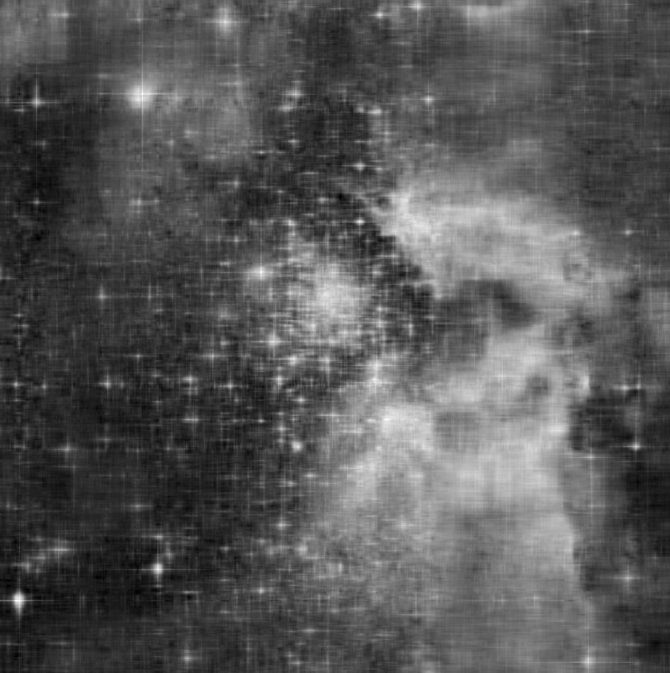
\includegraphics[width=\textwidth]{rank27.jpg}
\caption{Rank 27}
\end{subfigure}
\begin{subfigure}[b]{.25\textwidth}
\centering
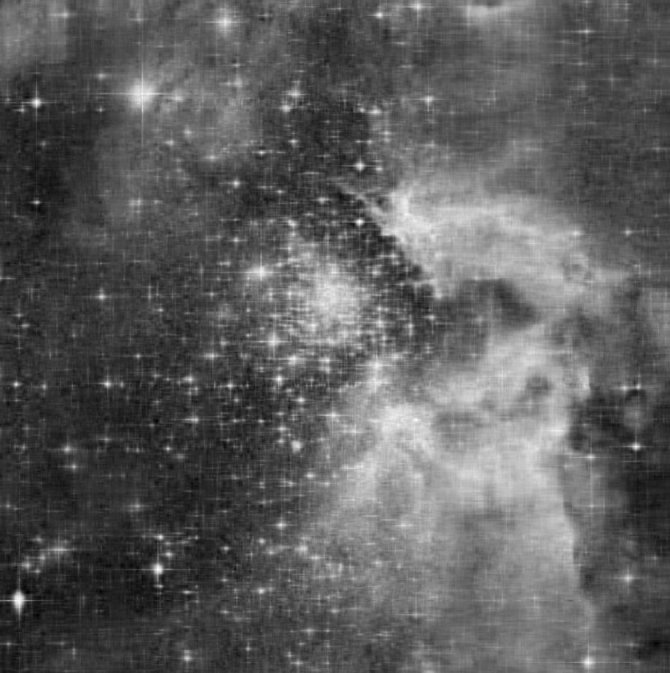
\includegraphics[width=\textwidth]{rank40.jpg}
\caption{Rank 40}
\end{subfigure}
\caption{Different rank approximations for SVD based compression.  Notice that higher rank is needed to resolve finer detail.}
\label{fig:rankvalues}
\end{figure}

To read in an image, convert it to black and white, and show it, use the code below.
Then use your function from Problem \ref{prob:svd_approx} to calculate an approximation.
%Enter the following into IPython (note that any image you might have will work):
\begin{lstlisting}
>>> import matplotlib.pyplot as plt
>>> from matplotlib import cm
>>> X = plt.imread('hubble_image.jpg')[:,:,0].astype(float)
>>> X.nbytes     #number of bytes needed to store X
>>> plt.imshow(X, cmap=cm.gray)
>>> plt.show()
\end{lstlisting}
\begin{comment}
Computing the SVD of your image is simple.
Remember to make the singular values a diagonal matrix before multiplying.
\begin{lstlisting}
>>> U,s,Vt = svd(X, full_matrices=False)
>>> S = sp.diag(s)
\end{lstlisting}
In the next code block, $n$ represents the desired rank of the output.
\begin{lstlisting}
>>> n = 50
>>> u1, s1, vt1 = U[:,0:n], S[0:n,0:n], Vt[0:n,:]
>>> Xhat = u1.dot(s1).dot(vt1)
>>> (u1.nbytes + np.diag(s1).nbytes + vt1.nbytes) - X.nbytes   #should be negative
>>> plt.imshow(Xhat)
>>> plt.show()
\end{lstlisting}
\end{comment}

Recall that the error between the best rank $s$ approximation $\widehat{A_s}$ to $A$ with respect to the induced 
2-norm is given by
$$
\|A - \widehat{A_s}\|_2 = \sigma_{s+1},
$$
where $\sigma_{s+1}$ is the $(s+1)$-th singular value of $A$. 

\begin{problem}
Using your \li{svd_approx} function from Problem \ref{prob:svd_approx}, write a function \li{lowest_rank_approx} that takes as input a matrix $A$ and a positive number $e$ and returns
the lowest rank approximation of $A$ with error less than $e$ (with respect to the induced 2-norm).
\end{problem}

\begin{problem}
Using your \li{svd_approx} function from Problem \ref{prob:svd_approx}, write a function \li{compress_img} that accepts two parameters \li{filename} and \li{k}. Your function should plot the original image and the best rank k approximation of the original image. Your output should be similar to Figure \ref{fig:compressed_image}.

At times, \li{plt.imshow} does not behave as expected when being passed RGB values between 0 and 255. It behaves much better when being passed numbers between 0 and 1. Additionally, since the SVD provides an approximation, it is possible that the SVD will generate values slightly outside the valid range of RGB values. To remedy this, use masks as discussed in the NumPy and SciPy lab. 

\begin{figure}[H]
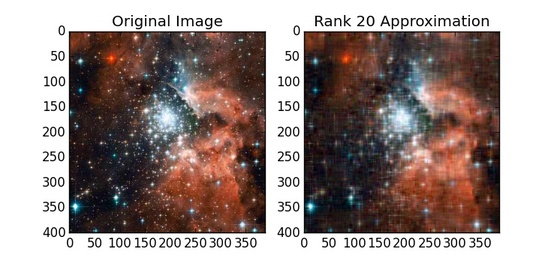
\includegraphics[width=\textwidth]{compressed.jpg}
\caption{Correct output for the best rank 20 approximation.}
\label{fig:compressed_image}
\end{figure}
\end{problem}
